%!TEX root = ../../../adrien_gomar_phd.tex

The mesh considered to compute this
CROR configuration is a single-blade passage meshed
with an O4H topology show in Fig.~\ref{fig:dream_mesh}. This is a classical
topology for turbomachinery computations that is here applied to 
a CROR.
\begin{figure}[htb]
  \centering
  \subfigure[Mesh topology]{
    \label{fig:dream_mesh}
    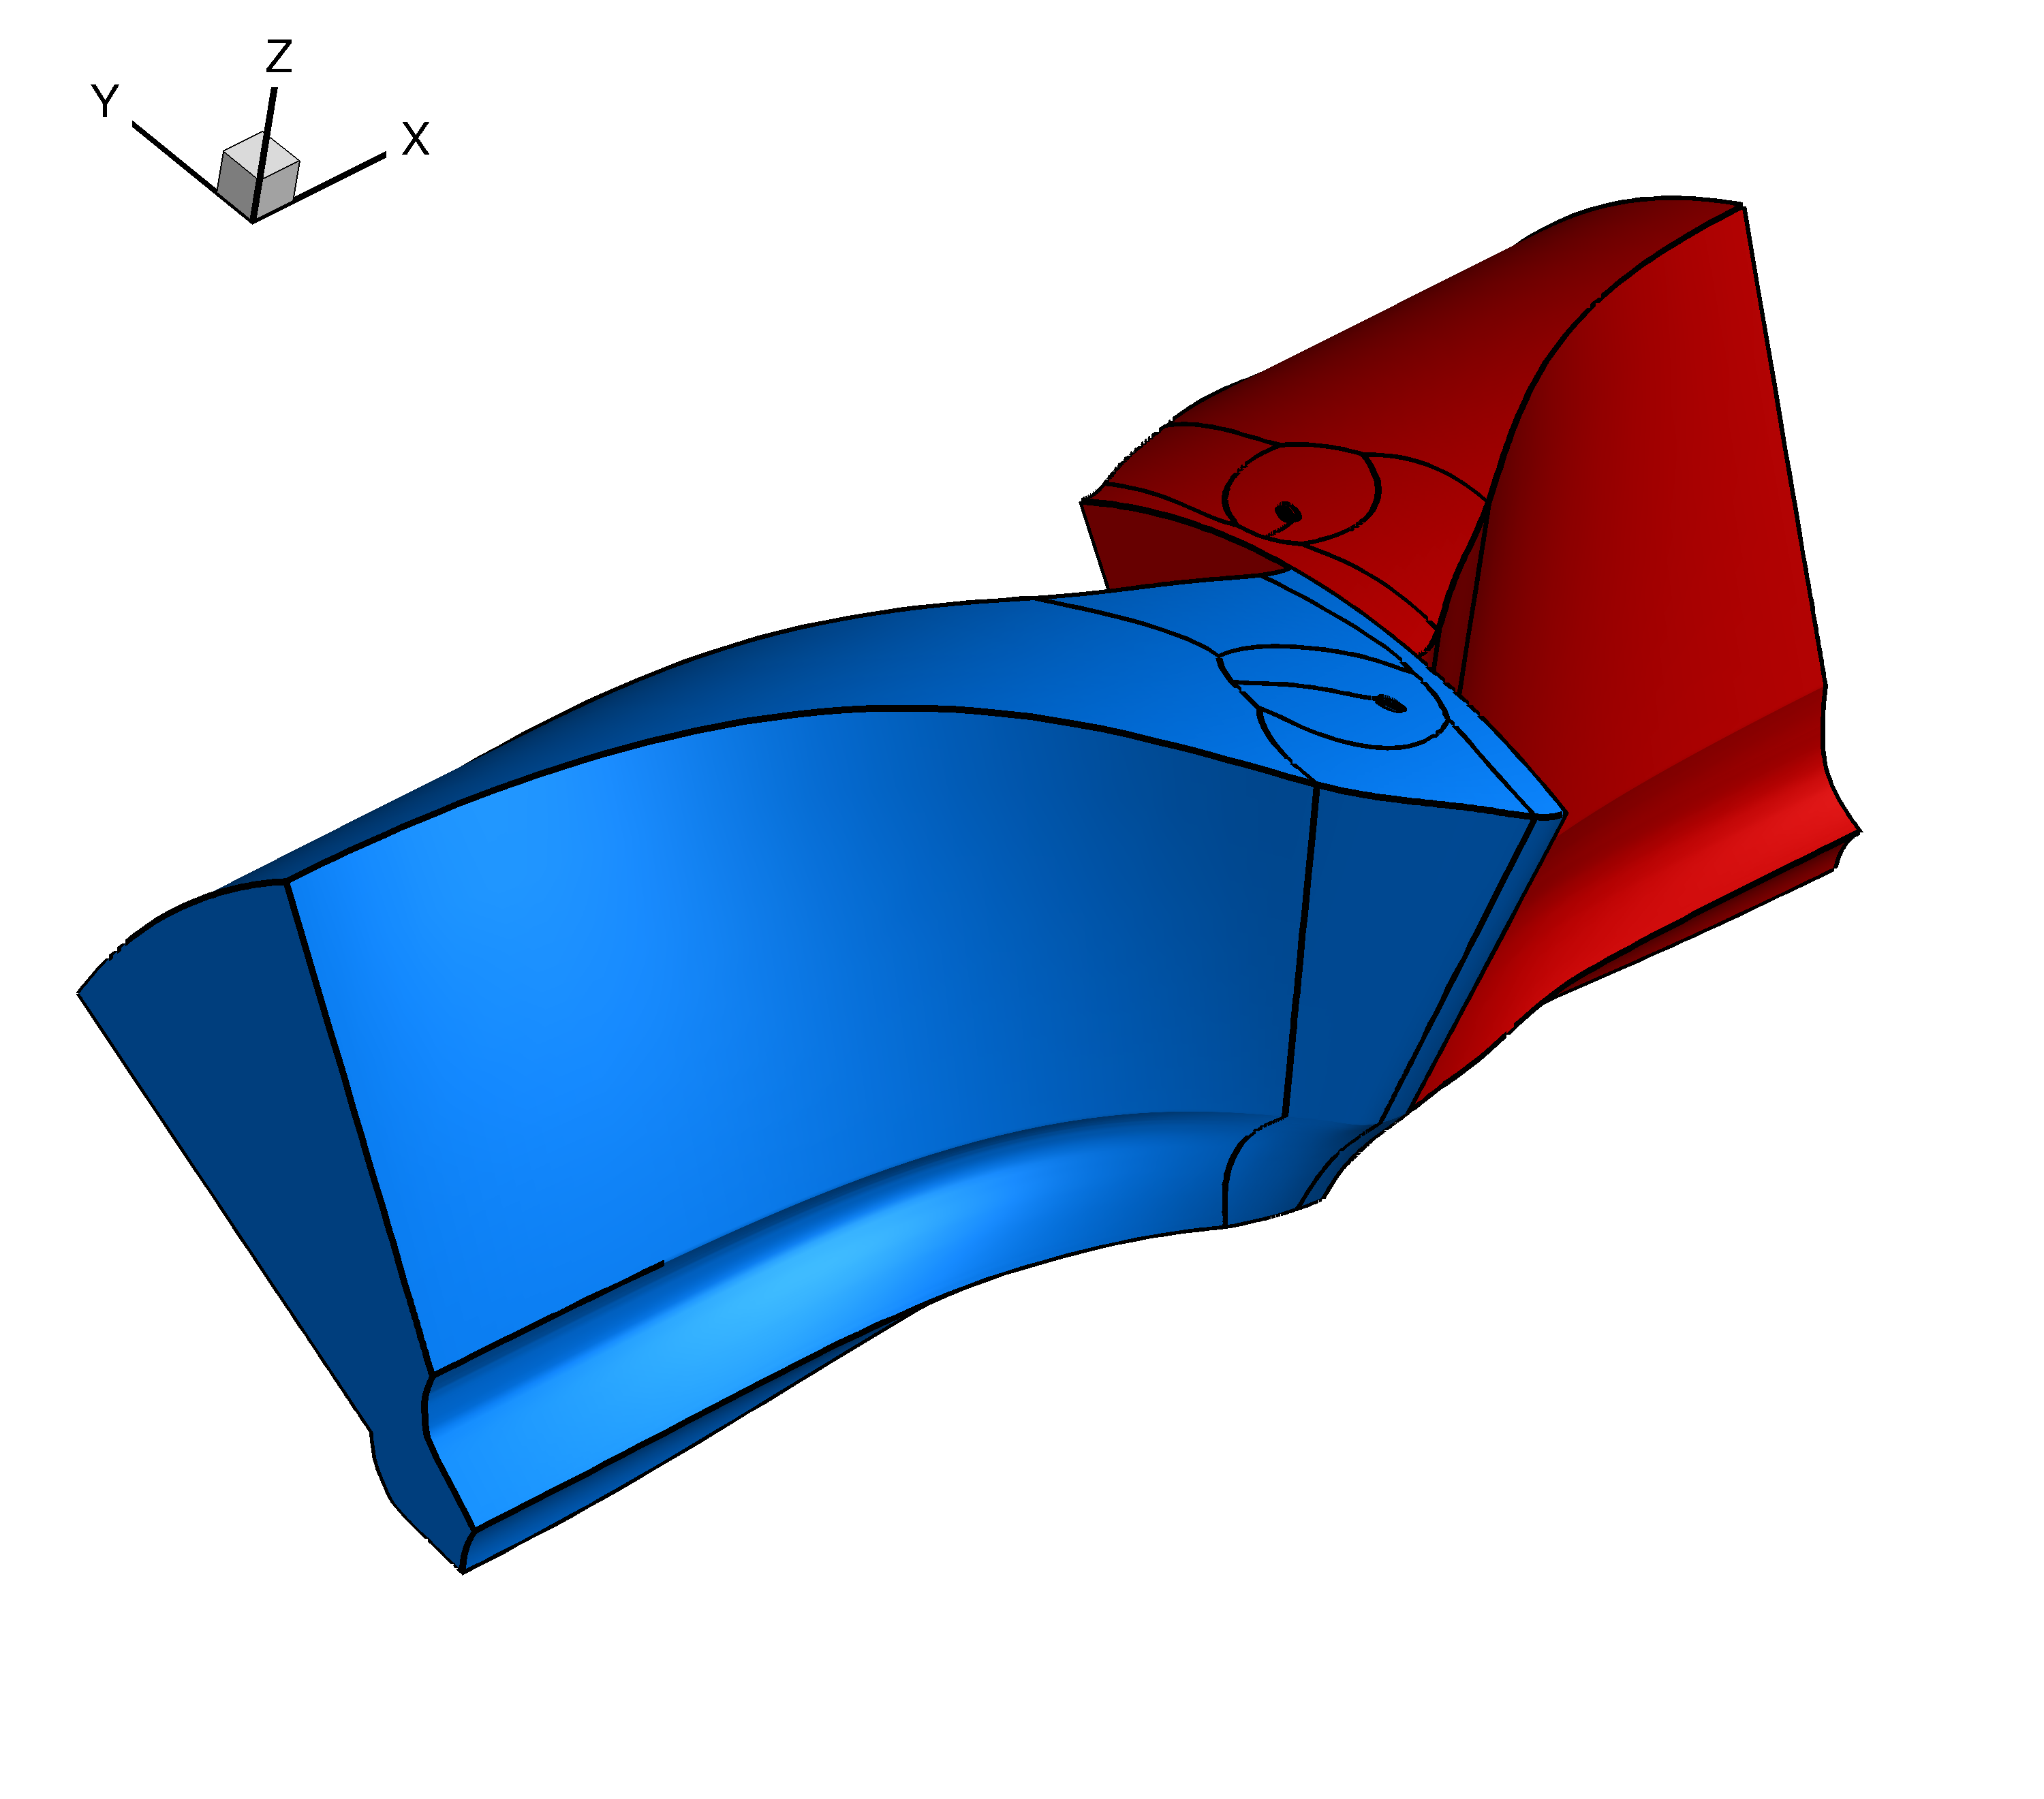
\includegraphics[width=.4\textwidth]{dream_mesh.png}}
  \subfigure[Far-field domain]{
    \label{fig:dream_farfield}
    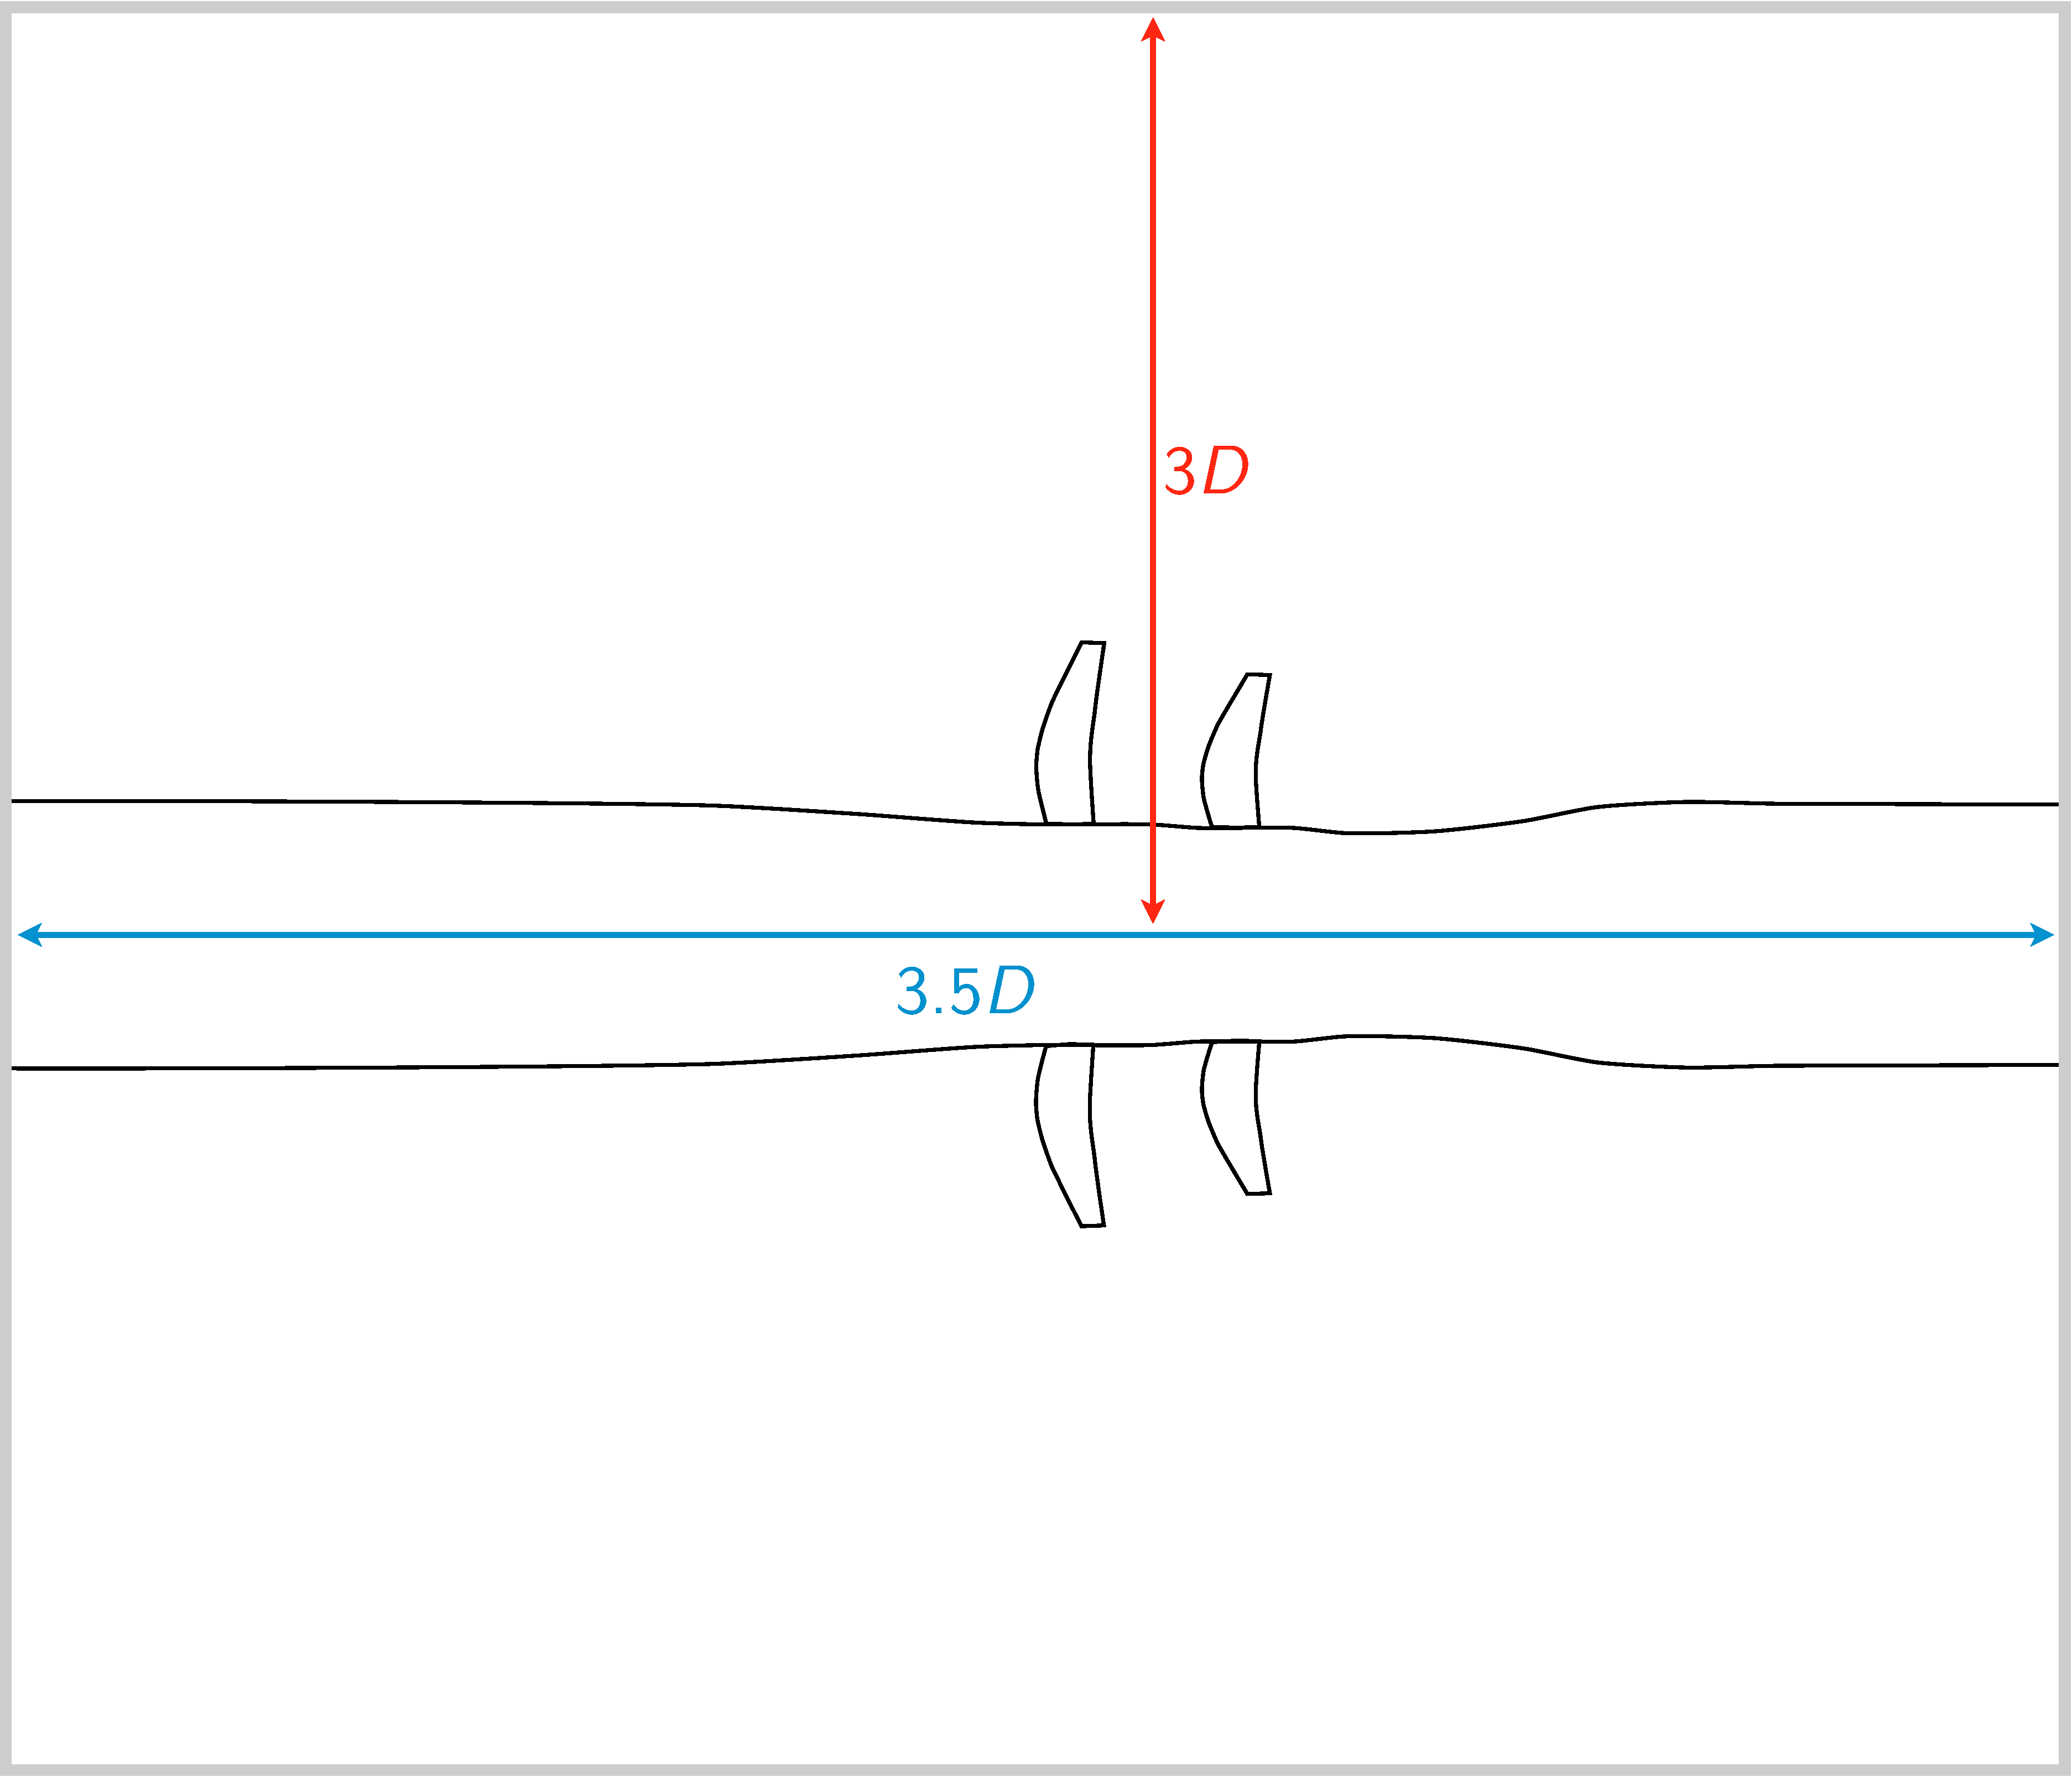
\includegraphics[width=.4\textwidth]{dream_farfield.pdf}}
  \caption{Computational domain considered.}
\end{figure}

As this last is not shrouded, a sufficiently large
far-field domain is taken to ensure a minimum influence
of the boundary conditions.
The computational domain is shown in Fig.~\ref{fig:dream_farfield}.
The radial extent is $3D$ while the axial one is $3.5D$.
\citet{Peters2012} consider an axial extent of $7.5D$
with a radial extent of $4D$ while \citet{Zachariadis2011}
consider $2.5D$ and $3.6D$, respectively. We are thus in 
the mid-range of the values taken in the literature.

As highlighted by underlined text in Fig.~\ref{fig:dream_farfield},
the boundary conditions used are: (i)~adiabatic walls
for the blades and the shroud (or spinner) and (ii)~constant
stagnation values used at the far-field.

Turbulence is modeled using the one-equation model of
\citet{Spalart1992}.  Roe's scheme~\cite{Roe1981} along with a 
second-order MUSL extrapolation 
is used to compute the convective fluxes.
The maximum CFL number is set to~10 for the steady 
computations and the HB simulations.
